\begin{frame}[t]{Introduction}
  \vspace{-0.70cm}
  \begin{center}
    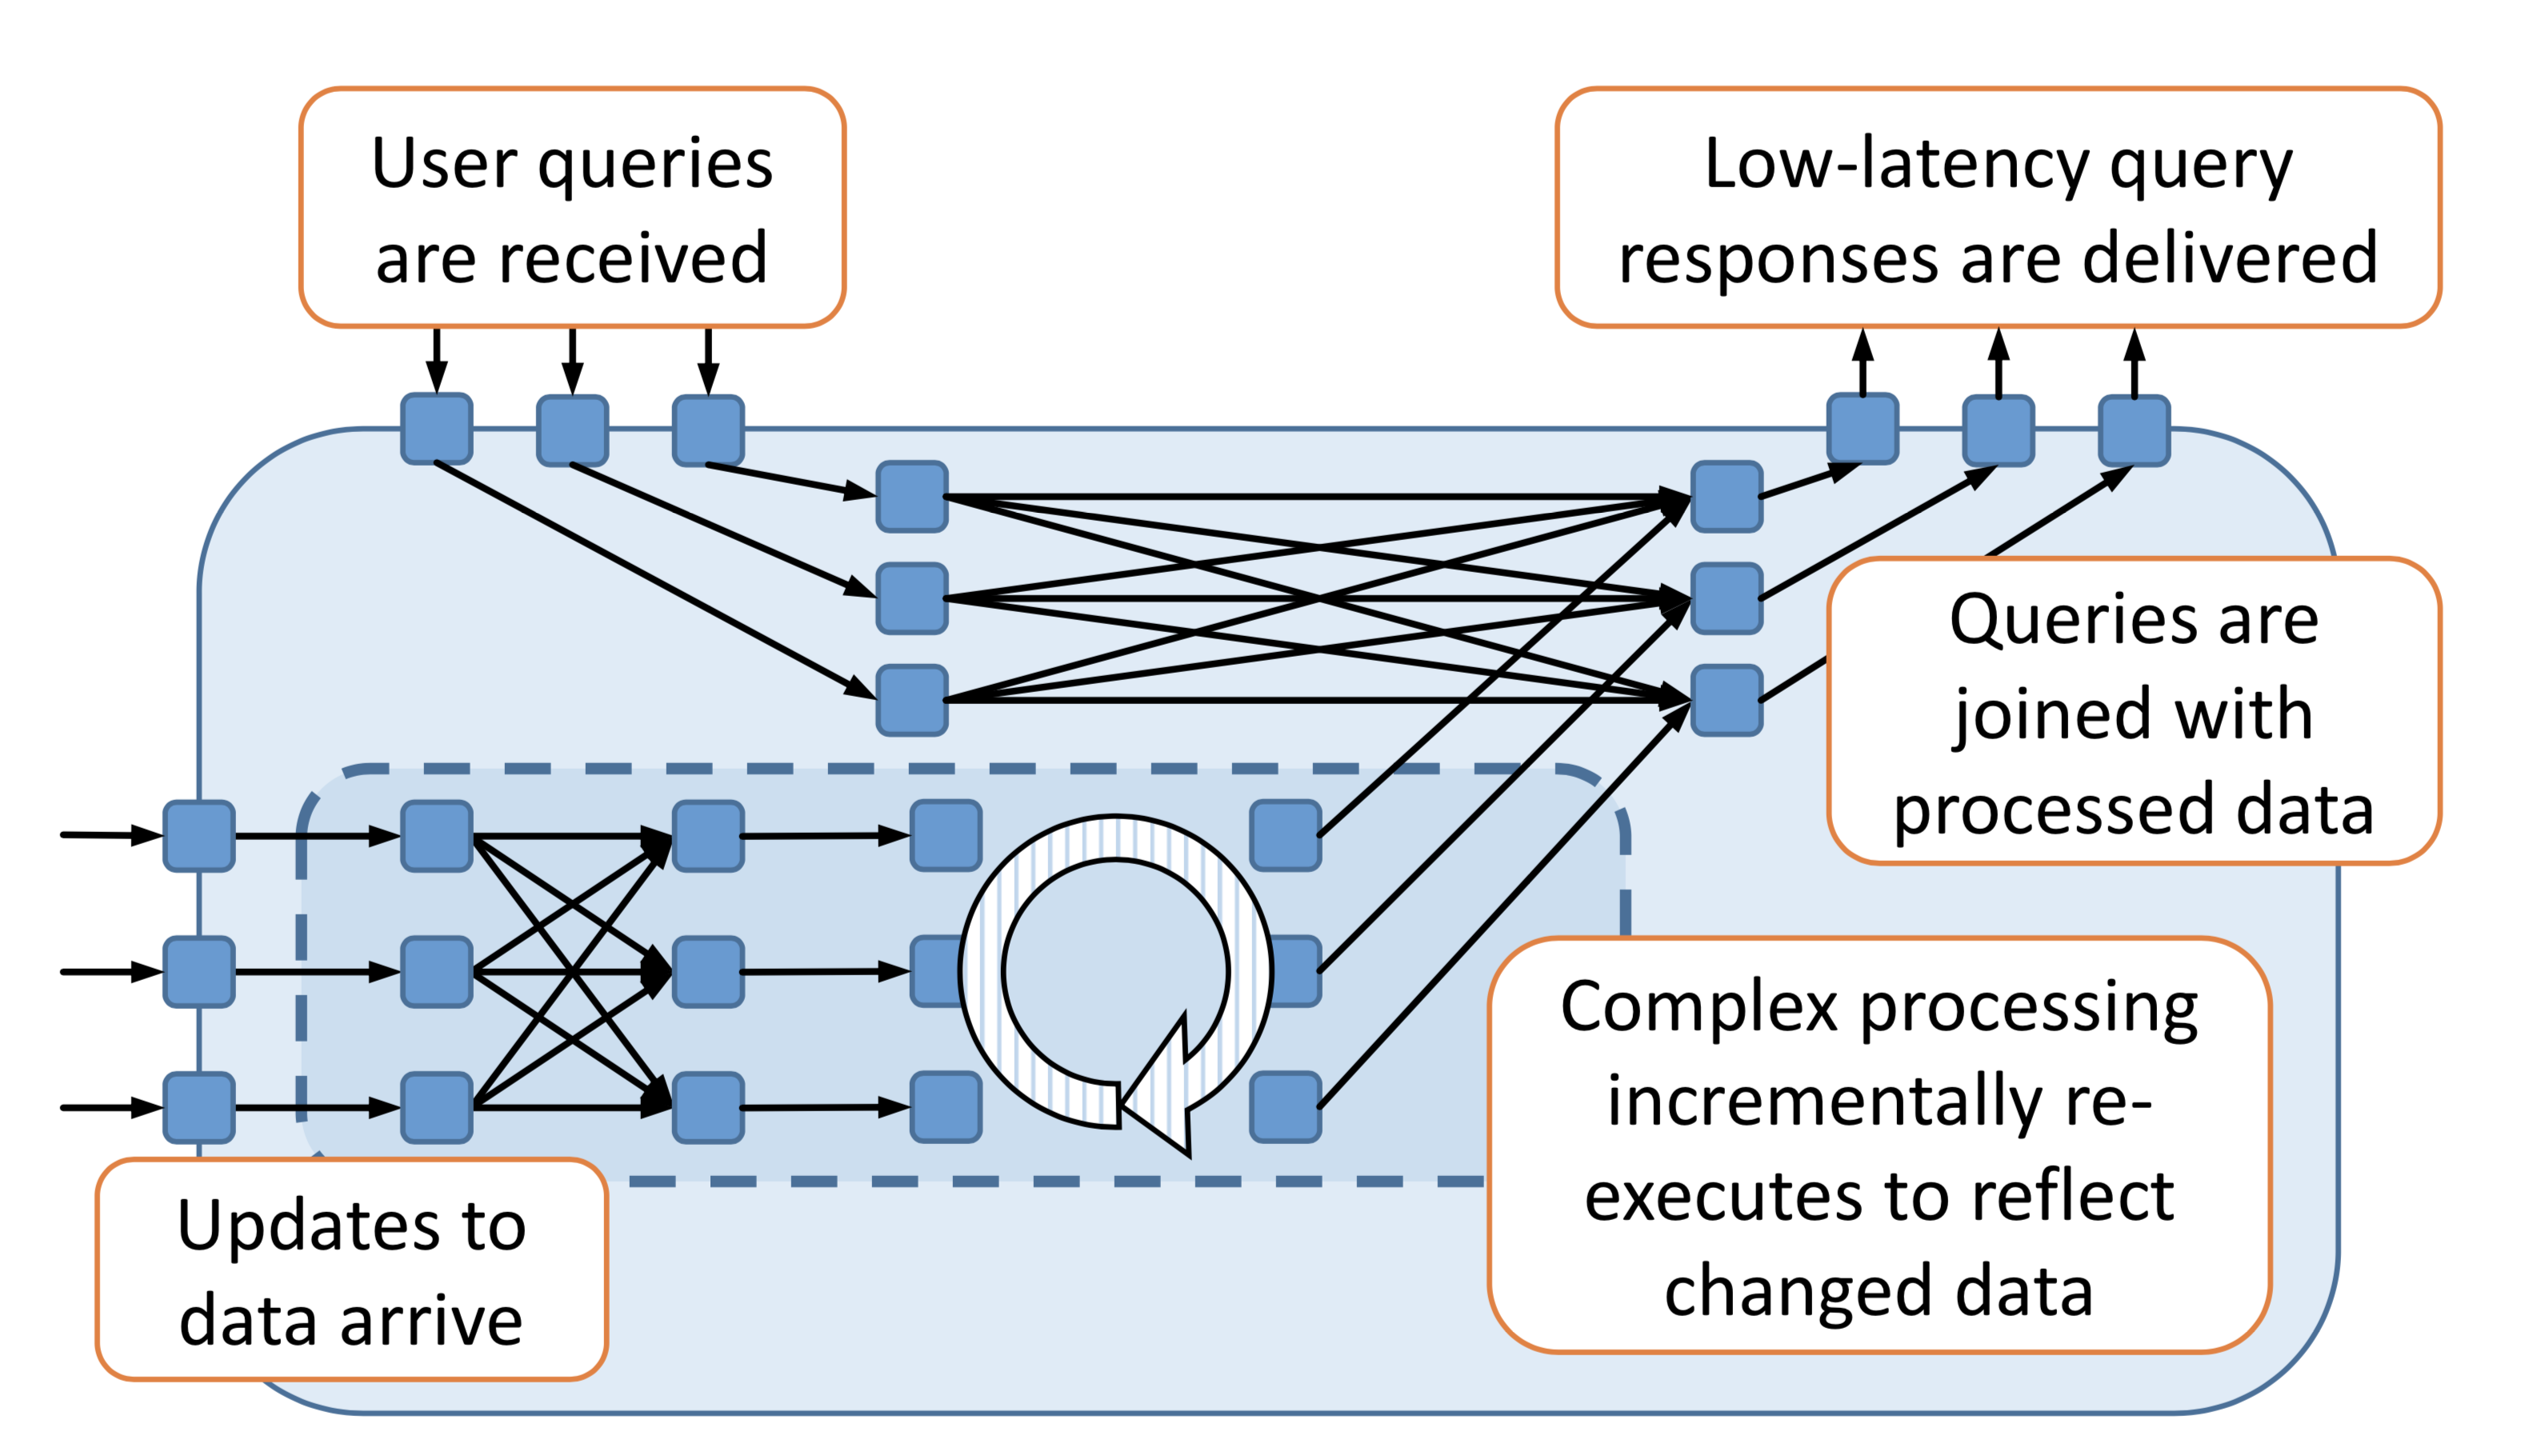
\includegraphics[width=0.76\textwidth]{1}
  \end{center}

  \pause
  \begin{columns}[t]
    \hspace{0.09\textwidth}
    \column{0.30\textwidth}
      \textbf{Batch}
      \begin{itemize}
        \item Iteration
        \item Consistency
        \item Poor latency
      \end{itemize}
    
    \column{0.30\textwidth}
      \textbf{Stream}
      \begin{itemize}
        \item No iteration
        \item No consistency
        \item Low latency
      \end{itemize}

    \column{0.30\textwidth}
      \textbf{Graph}
      \begin{itemize}
        \item Iteration
        \item Vertex-oriented Programming
      \end{itemize}
  \end{columns}
\end{frame}

\begin{frame}[t]{Introduction}
  \vspace{0.25cm}

  \begin{itemize}
    \setlength\itemsep{0.15cm}
    \item General purpose system
    \item Support high-level programming models
    \item Iteration on real-time data
    \item Supports interactive queries on fresh,\\ consistent view of results
    \item Low latency -- specialized system performance
  \end{itemize}
\end{frame}

\begin{frame}[t]{\emph{Timely} Dataflow}
  \begin{center}
    Dataflow programming primitives based on \emph{time}
  \end{center}

  \begin{itemize}
    \setlength\itemsep{0.15cm}
    \item Structured Loops
    \item Stateful vertices
    \item Notification for vertices on iteration completion
  \end{itemize}

  \vspace{0.25cm}
  \begin{center}
    \begin{tikzpicture}[->,>=stealth',shorten >=1pt,auto,node distance=2cm,
      thick,main node/.style={circle,draw,font=\sffamily\Large\bfseries}]

      \node[main node] (a) {A};
      \node[main node] (b) [right of=a] {B};
      \node[main node] (c) [right of=b] {C};
      \node[main node] (d) [below left of=c] {D};
      \node[main node] (e) [right of=c] {E};
      \path[every node/.style={font=\sffamily\small}]
      (a) edge (b) 
      (b) edge (c) 
      (c) edge (d) 
      (d) edge (b)
      (c) edge (e);
    \end{tikzpicture}
  \end{center}
\end{frame}

\begin{frame}[t]{Timely Dataflow - Graph Structure}
  \vspace{-0.5cm}
  \begin{center}
    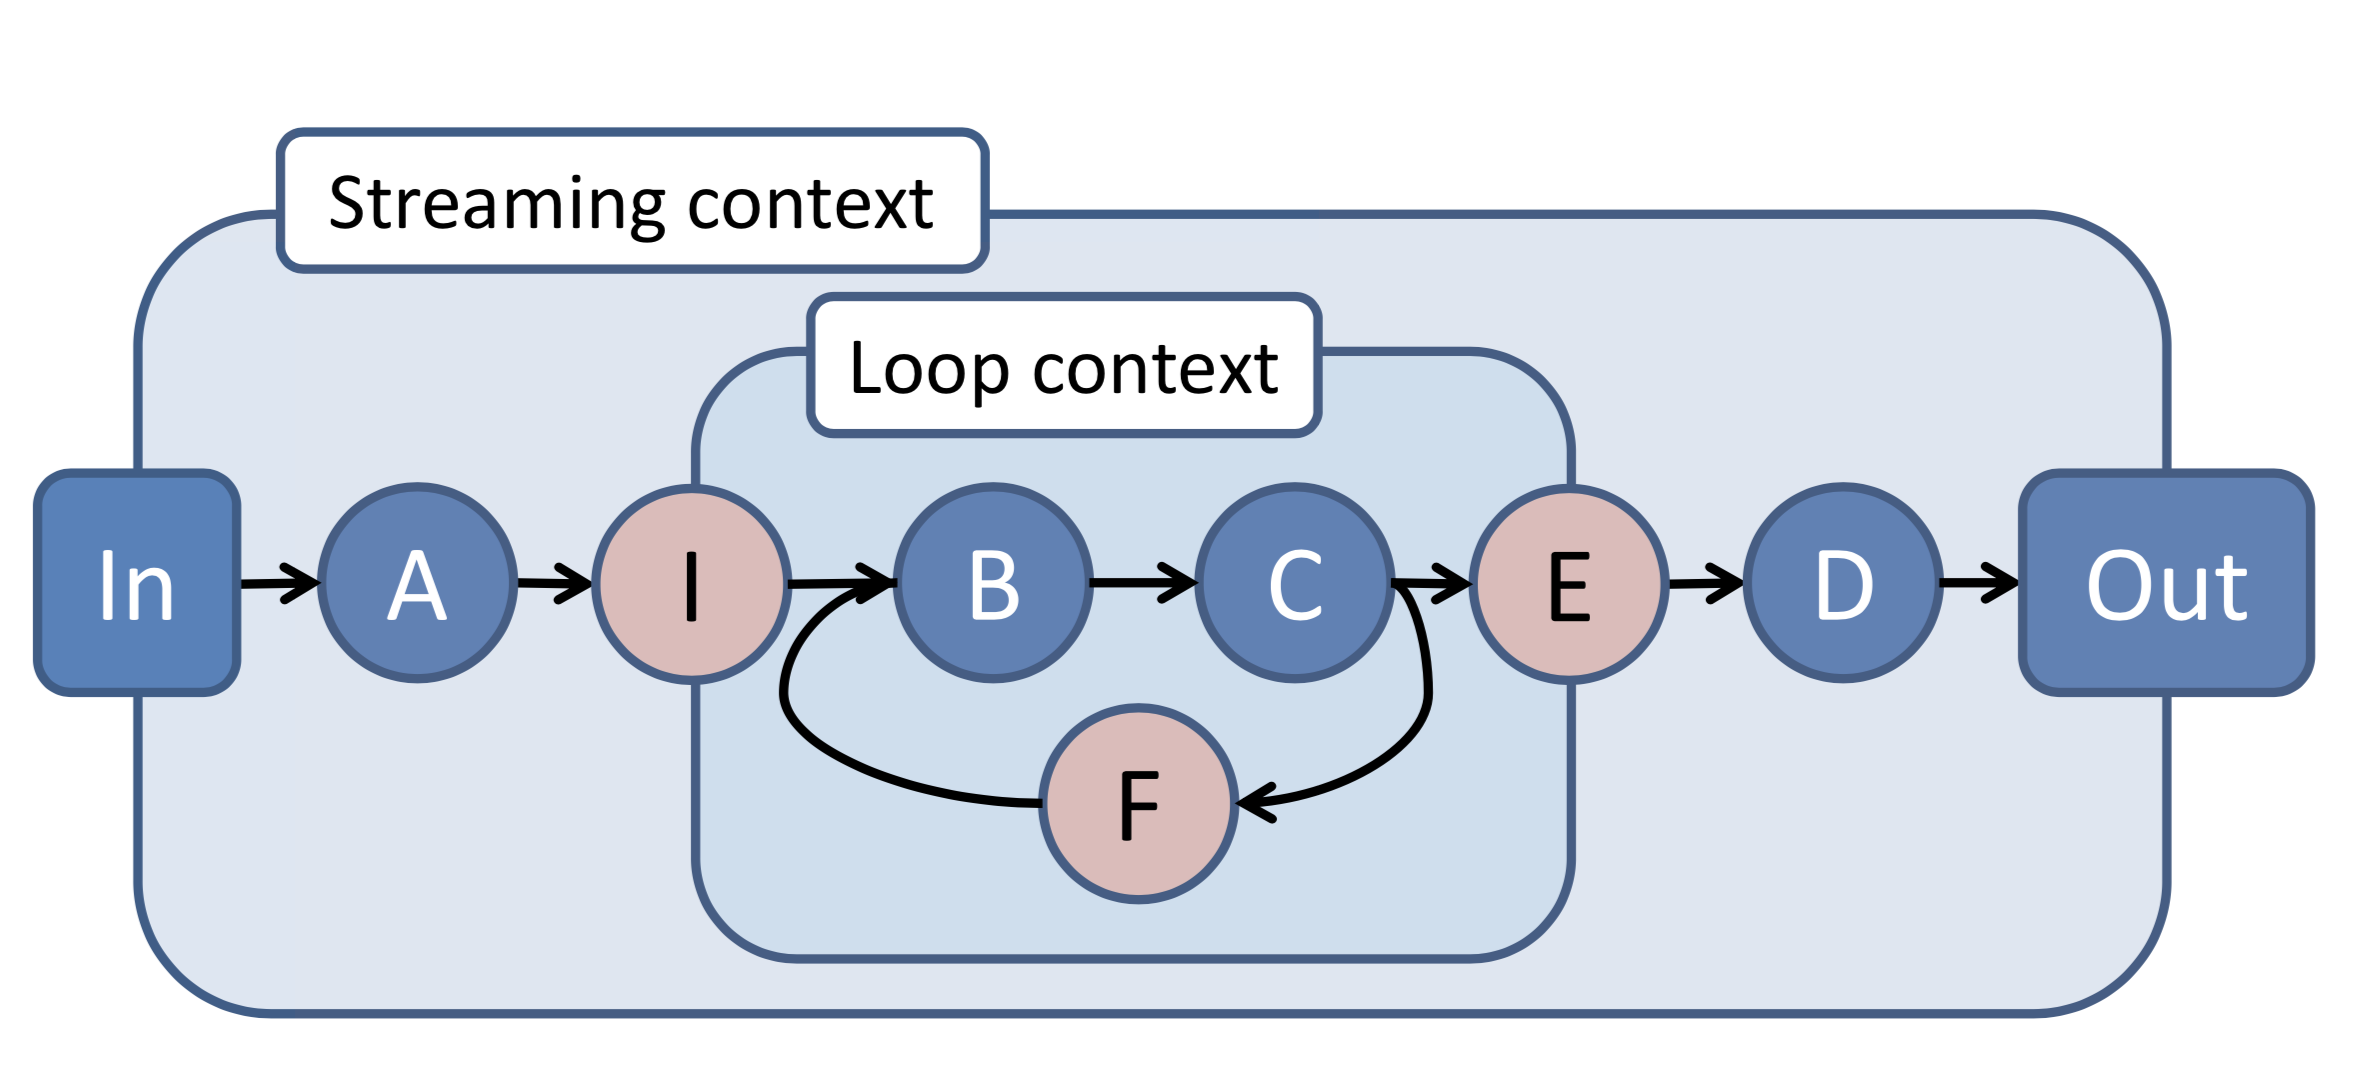
\includegraphics[width=0.85\textwidth]{2}
  \end{center}

  \vspace{-0.5cm}
  \begin{itemize}
    \setlength\itemsep{0.25cm}
    \item Time epoch on every input
    \item Streaming Context - Process data and pass
    \item Loop Context
    \begin{itemize}
      \setlength\itemsep{0.15cm}
      \item Loop - Ingress (I) $\Rightarrow$ Feedback (F) $\Rightarrow$ Egress (E)
      \item Monitors progress
    \end{itemize}
  \end{itemize}

\end{frame}

\begin{frame}[t]{Timely Dataflow - Concurrency Primitives}

  \vspace{0.5cm}
  \begin{center}
    \begin{tikzpicture}[->,>=stealth',shorten >=1pt,auto,node distance=2cm,
      thick,main node/.style={circle,draw,font=\sffamily\Large\bfseries}]

      \node[main node] (u) {$u$};
      \node[main node] (v) [right of=u] {$v$};

      \path[every node/.style={font=\sffamily\small}]
      [->] (u) edge (v);
    \end{tikzpicture}
  \end{center}

  \vspace{0.5cm}
  Vertices register callbacks \\
  \vspace{0.25cm}
  $v$.\textsc{OnRecv}($e$: Edge, $m$: Message, $t$: Timestamp) \\
  $v$.\textsc{OnNotify}($e$: Edge, $m$: Message, $t$: Timestamp) \\

  \vspace{0.75cm}
  Vertices generate events \\
  \vspace{0.25cm}
  $this$.\textsc{SendBy}($e$: Edge, $m$: Message, $t$: Timestamp) \\
  $this$.\textsc{NotifyAt}($t$: Timestamp) \\

\end{frame}

\begin{frame}[t]{Timely Dataflow - Concurrency Primitives}

  \vspace{0.5cm}
  \begin{center}
    \begin{tikzpicture}[->,>=stealth',shorten >=1pt,auto,node distance=2cm,
      thick,main node/.style={circle,draw,font=\sffamily\Large\bfseries}]

      \node[main node] (u) {$u$};
      \node[main node] (v) [right of=u] {$v$};

      \path[every node/.style={font=\sffamily\small}]
      [->] (u) edge (v);
    \end{tikzpicture}
  \end{center}

  \begin{itemize}
    \item \textsc{OnRecv} and \textsc{OnNotify} are queued, no strict ordering
    \vspace{0.15cm}
    \item Guarantee: \\ $v$.\textsc{OnNotify}$(t)$ is invoked only after no further invocations of
          $v$.\textsc{OnRecv}$(e,m,t')$, for $t' \leq t$
    \vspace{0.15cm}
    \item Constraint: \\ $v$.\textsc{SendBy}$(t')$ and $v$.\textsc{NotifyAt}$(t')$ \\
          such that $t' \geq t$
  \end{itemize}

\end{frame}

\begin{frame}[t]{Timely Dataflow - Timestamp}

  \begin{center}
    \Large{$(e\in\mathbb N, \langle c_1,\dots,c_k \rangle \in\mathbb N^k)$}
  \end{center}

  \vspace{0.25cm}
  Example: (epoch, counter) - $(1, \langle 0, 1, 2 \rangle)$

  \vspace{0.5cm}
  Vertex Behavior:
  \begin{itemize}
    \item Ingress  - $\langle c_1,\dots, {\color{blue} c_k} \rangle \Rightarrow \langle c_1,\dots, {\color{blue} c_k,  0} \rangle$
    \item Egress   - $\langle c_1,\dots, {\color{blue} c_k, c_{k+1}} \rangle \Rightarrow \langle c_1,\dots, {\color{blue} c_k}\rangle$
    \item Feedback - $\langle c_1,\dots,{\color{blue} c_k} \rangle \Rightarrow \langle c_1,\dots, {\color{blue} c_k, c_{k+1}} \rangle$
  \end{itemize}

  \vspace{0.25cm}

  Ordering: \\
  $ t_1 = (e_1, \vec{c_1}), t_2 = (e_2, \vec{c_2})$ \\
  $ t_1 < t_2$ $\iff$ $e_1 < e_2$ and $\vec{c_1} < \vec{c_2}$

\end{frame}

\begin{frame}[t]{Timely Dataflow - Progress Tracking}
  \vspace{0.25cm}

  Future timestamps constrained by,
  \begin{itemize}
    \item Unprocessed \emph{events} (\textsc{SendBy} and \textsc{NotifyAt})
    \item Graph structure
  \end{itemize}

  \only<2->{
    \vspace{0.5cm}
    \textbf{Pointstamp: $(t \in$ Timestamp, $l \in $ Edge $ \cup $ Vertex $ ) $}
  }

  \only<3->{
    \vspace{0.5cm}
    for, $v$.\textsc{SendBy($e,m,t$)}, pointstamp($m$) = $(t, e)$ \\
    \vspace{0.15cm}
    for, $v$.\textsc{NotifyAt($t$)}, pointstamp($m$) = $(t, v)$
  }

  \only<4->{
    \vspace{0.5cm}
    \textbf{Structure constraint induces ordering:}\\
    \vspace{0.15cm}
    $(t_1, l_1)$ \emph{could-result-in} $(t_2, l_2)$ $\iff$ $\exists$ path $\psi = \langle l_1, \dots, l_2 \rangle$ \\
    \vspace{0.15cm}
    such that $t_1$ is adjusted by each I, E or F, satisfies $\psi(t_1) \leq t_2$.
  }

\end{frame}

\begin{frame}[t]{Timely Dataflow - could-result-in}

  \vspace{0.15cm}

  \begin{center}
    \begin{tikzpicture}[->,>=stealth',shorten >=1pt,auto,node distance=2cm,
      thick,main node/.style={circle,draw,font=\sffamily\Large\bfseries}]

      \node[main node] (a) {A};
      \node[main node] (b) [right of=a] {B};
      \node[main node] (c) [right of=b] {C};
      \node[main node] (d) [below left of=c] {D};
      \node[main node] (e) [right of=c] {E};
      \path[every node/.style={font=\sffamily\small}]
      (a) edge (b) 
      (b) edge (c) 
      (c) edge (d) 
      (d) edge (b)
      (c) edge (e);
    \end{tikzpicture}
  \end{center}

  \vspace{0.15cm}

  Is there a path between D and E?

  \pause
  \vspace{0.15cm}
  $(1, A)$ \emph{could-result-in} $(1, E)$ ? \\
  \pause
  \vspace{0.15cm}
  $((1, 2), D)$ \emph{could-result-in} $((1, 4), C)$ ? \\
  \pause
  \vspace{0.15cm}
  $((3, 4), D)$ \emph{could-result-in} $(2, E)$ ? \\

\end{frame}

\begin{frame}[t]{Timely Dataflow - Single-Threaded Scheduler}
  \vspace{0.15cm}

  \begin{itemize}
    \item A set of \emph{active pointstamps} (at least 1 unprocessed event).
    \vspace{0.15cm}
    \item For each active poinstamp, maintains,
    \begin{itemize}
       \item \emph{occurrence count} - outstanding events.
       \item \emph{precursor count} - how many active poinstamps precede.
    \end{itemize}
    \vspace{0.15cm}
    \item Update \emph{occurrence count} for each event.
    \vspace{0.15cm}
    
    \pause
    \begin{exampleblock}{}
      \vspace{0.15cm}
      \begin{center}
        Scheduler is a simple message sorting function,\\
        to deliver notifications
      \end{center}
      \vspace{0.15cm}
    \end{exampleblock}
  \end{itemize}

\end{frame}

\begin{frame}{Visualizing the scheduler}

  \begin{center}
    \begin{tikzpicture}[->,>=stealth',shorten >=1pt,auto,node distance=2cm,
      thick,main node/.style={circle,draw,font=\sffamily\Large\bfseries}]

      \node[main node] (a) {A};
      \node[main node] (b) [right of=a] {B};
      \node[main node] (c) [right of=b] {C};
      \node[main node] (d) [below left of=c] {D};
      \node[main node] (e) [right of=c] {E};
      \path[every node/.style={font=\sffamily\small}]
      (a) edge (b) 
      (b) edge (c) 
      (c) edge (d) 
      (d) edge (b)
      (c) edge (e);
    \end{tikzpicture}
  \end{center}

  \vspace{0.15cm}
  \begin{center}
    \begin{tikzpicture}[->,>=stealth',shorten >=1pt,auto, node distance = 1cm and 2cm,
      thick,main node/.style={rectangle,draw,font=\scriptsize}]

      \node[main node] (c) {C.\textsc{SendBy}(\textunderscore, \textunderscore, (1, 5))};
      \node[main node] (d) [right=of a] {D.\textsc{NotifyAt}(1, 6)};
      \node[main node] (e) [right=of d] {E.\textsc{NotifyAt}(1)};
      \node[main node] (a) [below=of c] {A.\textsc{SendBy}(\textunderscore, \textunderscore, 2)};
      \node[main node] (b) [below right=of c] {B.\textsc{SendBy}(\textunderscore, \textunderscore, (2, 5))};

      \path[every node/.style={font=\sffamily\small}]
        (c) edge (d)
        (d) edge (e)
        (a) edge (b)
        (c) edge (b);
    \end{tikzpicture}
  \end{center}

\end{frame}

% \begin{frame}[t]{Timely Dataflow - Scheduler Lifecycle}
%   \vspace{0.5cm}

%   \begin{itemize}
%     \item Active pointstamps initialized at each input vertex, epoch 1. \\
%           Occurrence count = 1, Precursor count = 0
%     \vspace{0.15cm}
%     \item When epoch $e$ is marked complete, \\ 
%       a new active poinstamp at $e + 1$ is added.
%     \vspace{0.15cm}
%     \item Pointstamp for epoch $e$ is removed, \\ 
%       downstream notifications get delivered.
%     \vspace{0.15cm}
%     \item When input vertex is closed, all pointstamps are removed, \\
%       allowing downstream events to drain.
%   \end{itemize}
% \end{frame}
